% Options for packages loaded elsewhere
\PassOptionsToPackage{unicode}{hyperref}
\PassOptionsToPackage{hyphens}{url}
%
\documentclass[
]{article}
\usepackage{lmodern}
\usepackage{amssymb,amsmath}
\usepackage{ifxetex,ifluatex}
\ifnum 0\ifxetex 1\fi\ifluatex 1\fi=0 % if pdftex
  \usepackage[T1]{fontenc}
  \usepackage[utf8]{inputenc}
  \usepackage{textcomp} % provide euro and other symbols
\else % if luatex or xetex
  \usepackage{unicode-math}
  \defaultfontfeatures{Scale=MatchLowercase}
  \defaultfontfeatures[\rmfamily]{Ligatures=TeX,Scale=1}
\fi
% Use upquote if available, for straight quotes in verbatim environments
\IfFileExists{upquote.sty}{\usepackage{upquote}}{}
\IfFileExists{microtype.sty}{% use microtype if available
  \usepackage[]{microtype}
  \UseMicrotypeSet[protrusion]{basicmath} % disable protrusion for tt fonts
}{}
\makeatletter
\@ifundefined{KOMAClassName}{% if non-KOMA class
  \IfFileExists{parskip.sty}{%
    \usepackage{parskip}
  }{% else
    \setlength{\parindent}{0pt}
    \setlength{\parskip}{6pt plus 2pt minus 1pt}}
}{% if KOMA class
  \KOMAoptions{parskip=half}}
\makeatother
\usepackage{xcolor}
\IfFileExists{xurl.sty}{\usepackage{xurl}}{} % add URL line breaks if available
\IfFileExists{bookmark.sty}{\usepackage{bookmark}}{\usepackage{hyperref}}
\hypersetup{
  pdftitle={Simulation results},
  pdfauthor={Ella Orme},
  hidelinks,
  pdfcreator={LaTeX via pandoc}}
\urlstyle{same} % disable monospaced font for URLs
\usepackage[margin=1in]{geometry}
\usepackage{graphicx}
\makeatletter
\def\maxwidth{\ifdim\Gin@nat@width>\linewidth\linewidth\else\Gin@nat@width\fi}
\def\maxheight{\ifdim\Gin@nat@height>\textheight\textheight\else\Gin@nat@height\fi}
\makeatother
% Scale images if necessary, so that they will not overflow the page
% margins by default, and it is still possible to overwrite the defaults
% using explicit options in \includegraphics[width, height, ...]{}
\setkeys{Gin}{width=\maxwidth,height=\maxheight,keepaspectratio}
% Set default figure placement to htbp
\makeatletter
\def\fps@figure{htbp}
\makeatother
\setlength{\emergencystretch}{3em} % prevent overfull lines
\providecommand{\tightlist}{%
  \setlength{\itemsep}{0pt}\setlength{\parskip}{0pt}}
\setcounter{secnumdepth}{-\maxdimen} % remove section numbering
\usepackage{booktabs}
\usepackage{longtable}
\usepackage{array}
\usepackage{multirow}
\usepackage{wrapfig}
\usepackage{float}
\usepackage{colortbl}
\usepackage{pdflscape}
\usepackage{tabu}
\usepackage{threeparttable}
\usepackage{threeparttablex}
\usepackage[normalem]{ulem}
\usepackage{makecell}
\usepackage{xcolor}

\title{Simulation results}
\author{Ella Orme}
\date{}

\begin{document}
\maketitle

\hypertarget{resnmtf}{%
\section{ResNMTF}\label{resnmtf}}

\begin{figure}[H]

{\centering 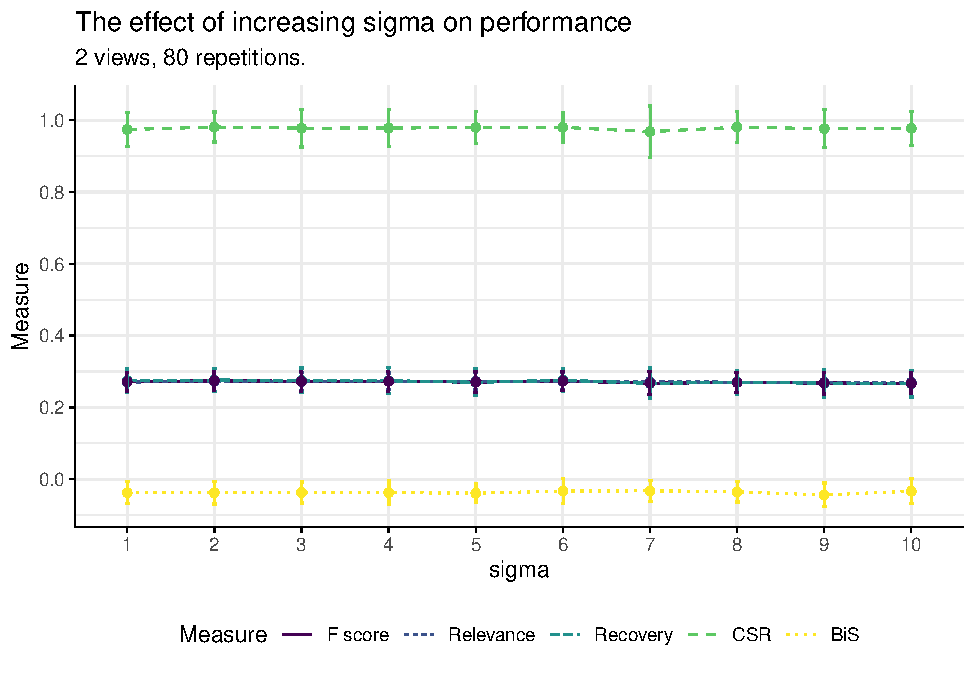
\includegraphics{issvd_results_files/figure-latex/unnamed-chunk-3-1} 

}

\caption{Simulation results for ResNMTF only.}\label{fig:unnamed-chunk-3}
\end{figure}

\begin{table}
\centering
\begin{tabular}[t]{llllllllllllllllllllll}
\toprule
\multicolumn{1}{c}{ } & \multicolumn{21}{c}{Per-comparrison wise error rate} \\
\cmidrule(l{3pt}r{3pt}){2-22}
  & 0 & 0.05 & 0.1 & 0.15 & 0.2 & 0.25 & 0.3 & 0.35 & 0.4 & 0.45 & 0.5 & 0.55 & 0.6 & 0.65 & 0.7 & 0.75 & 0.8 & 0.85 & 0.9 & 0.95 & 1\\
\midrule
F score & 0.0000 (0.0000) & 0.0000 (0.0000) & 0.0000 (0.0000) & 0.0000 (0.0000) & 0.0000 (0.0000) & 0.0000 (0.0000) & 0.0000 (0.0000) & 0.0003 (0.0028) & 0.0005 (0.0052) & 0.0004 (0.0042) & 0.0006 (0.0062) & 0.0007 (0.0073) & 0.0036 (0.0251) & 0.0126 (0.0659) & 0.0273 (0.1091) & 0.0260 (0.1045) & 0.0252 (0.1026) & 0.0242 (0.0924) & 0.0224 (0.0905) & 0.0240 (0.0905) & 0.0210 (0.0847)\\
Relevance & 0.0000 (0.0000) & 0.0000 (0.0000) & 0.0000 (0.0000) & 0.0000 (0.0000) & 0.0000 (0.0000) & 0.0000 (0.0000) & 0.0000 (0.0000) & 0.0006 (0.0057) & 0.0010 (0.0104) & 0.0008 (0.0083) & 0.0012 (0.0124) & 0.0015 (0.0146) & 0.0071 (0.0503) & 0.0253 (0.1317) & 0.0492 (0.1871) & 0.0465 (0.1769) & 0.0449 (0.1724) & 0.0484 (0.1848) & 0.0404 (0.1589) & 0.0426 (0.1552) & 0.0375 (0.1464)\\
Recovery & 0.0000 (0.0000) & 0.0000 (0.0000) & 0.0000 (0.0000) & 0.0000 (0.0000) & 0.0000 (0.0000) & 0.0000 (0.0000) & 0.0000 (0.0000) & 0.0002 (0.0019) & 0.0003 (0.0035) & 0.0003 (0.0028) & 0.0004 (0.0041) & 0.0005 (0.0049) & 0.0024 (0.0168) & 0.0084 (0.0439) & 0.0194 (0.0812) & 0.0185 (0.0783) & 0.0180 (0.0772) & 0.0161 (0.0616) & 0.0160 (0.0673) & 0.0179 (0.0726) & 0.0152 (0.0641)\\
CSR & 0.2500 (0.0000) & 0.2500 (0.0000) & 0.2500 (0.0000) & 0.2500 (0.0000) & 0.2500 (0.0000) & 0.2500 (0.0000) & 0.2500 (0.0000) & 0.2535 (0.0350) & 0.2535 (0.0350) & 0.2535 (0.0350) & 0.2535 (0.0350) & 0.2535 (0.0350) & 0.2570 (0.0492) & 0.2640 (0.0689) & 0.2768 (0.1007) & 0.2768 (0.1007) & 0.2768 (0.1007) & 0.2745 (0.0898) & 0.2768 (0.1007) & 0.2855 (0.1196) & 0.2768 (0.1007)\\
BiS & 0.0000 (0.0000) & 0.0000 (0.0000) & 0.0000 (0.0000) & 0.0000 (0.0000) & 0.0000 (0.0000) & 0.0000 (0.0000) & 0.0000 (0.0000) & 0.0039 (0.0387) & 0.0044 (0.0445) & 0.0045 (0.0446) & 0.0045 (0.0451) & 0.0046 (0.0458) & 0.0091 (0.0641) & 0.0171 (0.0844) & 0.0303 (0.1111) & 0.0304 (0.1117) & 0.0304 (0.1117) & 0.0294 (0.1078) & 0.0280 (0.1050) & 0.0377 (0.1219) & 0.0285 (0.1067)\\
\bottomrule
\multicolumn{22}{l}{\textsuperscript{a} 3 views, 100 repetitions.}\\
\end{tabular}
\end{table}

\hypertarget{correlation}{%
\section{Correlation}\label{correlation}}

\begin{tabular}[t]{lrr}
\toprule
  & BiS & CSR\\
\midrule
F score & 0.9825956 & 0.9776852\\
Relevance & 0.9799617 & 0.9723754\\
Recovery & 0.9845058 & 0.9817401\\
\bottomrule
\end{tabular}

\end{document}
